\documentclass[12pt, oneside]{report}

\usepackage[sfdefault]{roboto} 
\usepackage[T1]{fontenc}
\usepackage[utf8]{inputenc}
\usepackage[english,francais]{babel}

% ___________________________ A changer

\newcommand{\thedate}{}	% Date
\newcommand{\auteur}{InMoov}	% Auteur
\newcommand{\titre}{Documentation}
\newcommand{\typeDoc}{Électronique}

% _______________________________ No touch
%______________________________________________________________________________

\title{\titre}
\author{\auteur}
\date{\today}

%interactive tableofcontent and url
\usepackage{hyperref}
 
\usepackage[head=36pt,foot=30pt,top=3cm, bottom=3.5cm, outer=2cm, inner=2cm]{geometry}

% PKG : images
\usepackage{graphicx}
% PKG : color
\usepackage{xcolor}
% PKG : lipsum
\usepackage{lipsum}
% PKG : item 
\usepackage{enumitem}
\usepackage{pifont}
% PKG : position image avec H en parametre 
\usepackage{float}
% PKG : header and footer
\usepackage{lastpage} 
\usepackage{fancyhdr}
\pagestyle{fancy}

% ---- COLOR ---- %
\definecolor{gris}{rgb}{0.36,0.36,0.36}
\definecolor{bleu}{rgb}{0.1137,0.4941,0.5921}
\definecolor{gristitle}{rgb}{0.95,0.95,0.95}
\definecolor{vert}{rgb}{0.3,0.7,0.3}

\fancyhf{}
\lhead{\color{gris} \textbf{\titre}}
\rhead{
\includegraphics[width=4cm]{img_template/DVB_Banner.png}}
\rfoot{Page \thepage\ sur \pageref{LastPage}}

\begin{document}

\begin{titlepage}
	\centering
    \vspace*{0.5 cm}
   % \includegraphics[scale = 0.075]{bsulogo.png}\\[1.0 cm]	% University Logo
\begin{center}    \textsc{\Large   \typeDoc}\\[2.0 cm]	\end{center}% University Name
	\textsc{\Large \thedate  }\\[0.5 cm]				% Course Code
	\rule{\linewidth}{0.2 mm} \\[0.4 cm]
	{ \huge \bfseries \titre}\\
	\rule{\linewidth}{0.2 mm} \\[1.5 cm]
	
	\begin{minipage}{0.4\textwidth}
		\begin{flushleft} \large
			\end{flushleft}
			\end{minipage}~
			\begin{minipage}{0.4\textwidth}
            
			\begin{flushright} \large
			\emph{Écrit par :} \\
			\auteur  
		\end{flushright}
           
	\end{minipage}\\[2 cm]
	
	
\includegraphics[width=8cm]{img_template/DVB_Square.png}

\end{titlepage}

\tableofcontents

\chapter{Le résaux informatiqueleo}
    \section{Introduction}
        \subsection{Comment fonctionne Internet ?}
        \paragraph{}{Internet est le réseau informatique mondial accessible au public. C'est un réseau de réseaux, composé de millions de réseaux (publics, privés, universitaires, commerciaux,...) accessibles via des milliers de serveurs répartis partout dans le monde et communiquant entre eux par canaux de fibres optiques. }
        \textit{QU'EST CE QU'UN SERVEUR ??}
        
        \begin{figure}[h]
        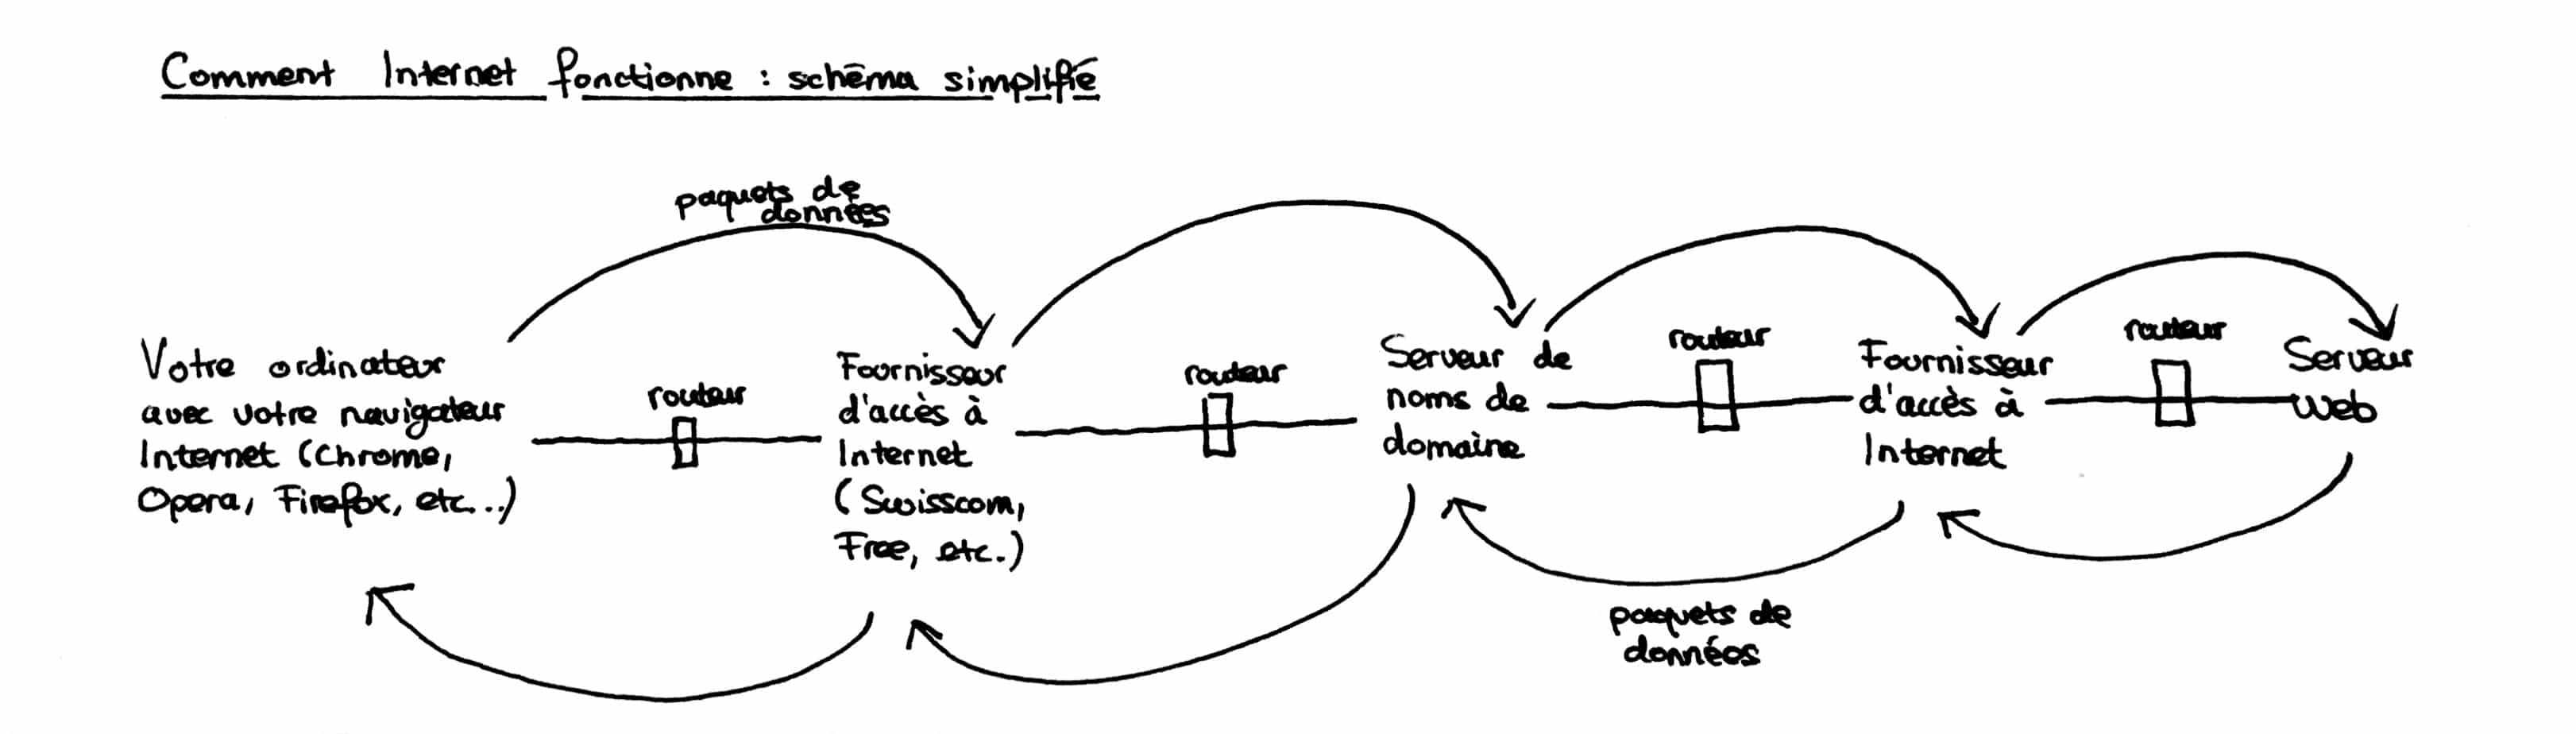
\includegraphics[scale = 0.18]{img_template/comment-internet-fonctionne.jpg}
        \centering
        \label{Fctn Internet}
        \end{figure}        
        
        \subsection{L'accès à Internet}
        \paragraph{}{Nous pouvons accéder à Internet par le biais de tous les appareils tels que téléphones portables, ordinateurs, tablettes qui ont cette fonctionnalité. Le modem, fourni par le fournisseur d'accès, est l'élément essentiel qui apporte l'accès à Internet dans un LAN (Local Area Network) : il reçoit directement les informations émises par le serveur via la fibre optique. Si on prend l'exemple d'un réseau dans une maison, ce qu'on appelle communément la "box" va jouer ce rôle de modem. Le routeur quant à lui, en se connectant au modem, est celui qui va transmettre la connexion Internet à tous les appareils de la maison, que ce soit en filaire, via un câble Ethernet, ou via Wi-Fi (le modem ne permettant qu'une unique connexion filaire, c'est la raison pour laquelle une très grande partie des foyers utilise un routeur aujourd'hui).\\Cependant, si on décide de se connecter à Internet en utilisant des données cellulaires, le signal doit être envoyé à partir du câble optique vers une tour de téléphonie cellulaire. C'est à partir de cette dernière que le signal atteint notre téléphone mobile sous forme d'ondes électromagnétiques.}
        \section{Ensemble de protocole de communication : \\ WiFi}
        \subsection{Port}
        \paragraph{}{Un port logiciel permet de différencier entre plusieurs programmes informatiques qui dans leur tour écoutent ou émettent des informations à ces ports. Ceux-ci sert localement à identifier un processus.
        
\paragraph{}Il y a aussi les sockets, identifiant unique dans un réseau, c’est le résultat de la concaténation de l’adresse IP et le numéro du port. 
L'adresse IP sert donc à identifier de façon unique un ordinateur sur le réseau tandis que le numéro de port indique l'application à laquelle les données sont destinées. De cette manière, lorsque l'ordinateur reçoit des informations destinées à un port, les données sont envoyées vers l'application correspondante. S'il s'agit d'une requête à destination de l'application, l'application est appelée application serveur. S'il s'agit d'une réponse, on parle alors d'application cliente.
\paragraph{}Il existe une convention pour attribuer des numéros des ports à leur fonctions et utilités :
Les numéros des ports du serveur varient généralement entre 0 et 1023 (well known ports).
Alors que pour les clients, les ports sont choisis aléatoirement parmi ceux disponibles donc ne seront jamais compris entre 0 et 1023 car ils sont déjà pris.
}
        \section{Protocole de télécommunications}
        \subsection{User Datagram Protocol : UDP}
        \paragraph{Introduction}{Le Protocole de Datagramme Utilisateur est un des principaux protocoles de télécommunications utilisés par Internet. Il permet la transmission de données (sous formes de datagrammes d'où son nom) de manière très simple entre deux entités, chacune étant définie par une adresse IP et un numéro de port. On peut ainsi avoir un échange d'informations entre un client et un serveur. Aucune communication préalable n'est requise pour établir une connexion, au contraire de TCP (qui utilise le procédé de handshaking)}
        \paragraph{Structure de datagramme}{Le terme de datagremme (aussi connu sous le nom de paquet) est utilisé pour décrire un bloc de données IP. Chaque datagramme IP contient un ensemble spécifique de champs dans un ordre précis afin que le destinataire sache comment décoder et lire le flux de données recu.}
        \paragraph{}{L'entête de l'UDP est constitué de 8 bites. On y trouve le port source codé sur 16bits, le port destinataire, également sur 16bits, la longueur (\textit{ie.} la taille de l'entête et des données) et le Checksum (somme de contrôle) qui représente la validité du paquet incluant les adresses IP source et destinatiare.}
        \paragraph{}{A la suite du UDP Header, on retrouve l'UDP Data où l'on va ainsi envoyer des données au récepteur.}
\chapter{Microcontrôleur avec connexion WiFi : \\ ESP 8266}
\section{Introduction}
        \paragraph{}{L'ESP8266 fonctionne dans deux modes: Station (STA) et Access Point (AP). En bref, le mode AP permet de créer son propre réseau et d’y connecter d’autres appareils (votre téléphone), tandis que le mode STA permet à l’ESP8266 de se connecter à un réseau Wi-Fi (créé par votre routeur sans fil). Ainsi, une caractéristique importante de l'ESP8266 est qu'il peut fonctionner en tant que client ou en point d'accès ou même les deux.
        }
\section{Configuration}
        \paragraph{}
\chapter{Système d'exploitation pour la robotique : \\ ROS}
\section{Introduction}
        \paragraph{}
\end{document}

